%%%%%%%%%%%%%%%%%%%%%%%%%%%%%%%%%%%%%%%%%%%%%%%%%%%%%%%%%%%%%%%%%%%%%%%%
% Plantilla TFG/TFM
% Escuela Politécnica Superior de la Universidad de Alicante
% Realizado por: Jose Manuel Requena Plens
% Contacto: info@jmrplens.com / Telegram:@jmrplens
%%%%%%%%%%%%%%%%%%%%%%%%%%%%%%%%%%%%%%%%%%%%%%%%%%%%%%%%%%%%%%%%%%%%%%%%

\chapter{Estado de arte}
En este apartado se va a presentar el impacto y el beneficio de la tecnología entrando, cada vez más, en el campo práctico de los servicios sociales.
\vspace{1em}
\par La tecnología ha revolucionado nuestra forma de consumir, de relacionarnos y de informarnos. Donde tampoco han sido ajenos a la evolución de la tecnología, es en el ámbito de los servicios sociales. Sin embargo, comparándolo con otros sectores mucho más maduros y con más presupuesto como la banca o el comercio, el sector social parece no haber sido capaz de adoptar o tener acceso a toda la tecnología que ya está desarrollada, afectando negativamente al servicio humano que se pretende dar.
\vspace{1em}
\par La tecnología en los servicios sociales tiene un papel cada vez mayor, éste puede adoptar muchas formas, como el uso de inteligencia artificial, los sistemas de gestión de casos y/o servicios especialmente desarrollados para hacer uso de la tecnología de asistencia. Como se estaba explicando, éstos avances tecnológicos pueden ayudar a mejorar la planificación, gestión y prestación de servicios sociales, pero también es importante comprender los desafíos que plantea la digitalización, como la falta de conocimiento sobre las nuevas tecnologías, su costo y cómo garantizar la protección de la privacidad y la seguridad.
\vspace{1em}
\par Aquí entraría en juego la Universidad de Alicante con su plan formativo de Ingeniería Informática, formando personal con los conocimientos y habilidades necesarias para ayudar acotar, acortar y amortiguar los miedos que suponen en este sector la aproximación a la tecnología.
% --------------------------------------------------------------
% --------------------------------------------------------------
% --------------------------------------------------------------
\clearpage
\section{La importancia de la tecnología en el campo social}
Puede que la crisis del COVID-19 pueda resultarnos nueva, sin embargo las crisis medioambientales y de salud han sido una constante en nuestro planeta. Éstas siempre han superado las agendas planificadas y los objetivos establecidos de las organizaciones comunitarias para continuar ejerciendo labores de manera tradicional y más importante aún, para coordinar asistencia social y llegar a los más necesitados. Por ejemplo en Puerto Rico se han experimentado fenómenos que han derrotado cualquier intento de gestión, desde el Huracán María hasta el terremoto de 2020, resultando en una falta de atención a las necesidades sociales.
\vspace{1em}
\par Como consecuencia de este tipo de crisis, las organizaciones de impacto comunitario se ven obligadas a redirigir sus esfuerzos hacia nuevas maneras de alcanzar sus objetivos. Esta problemática, a su vez, se extiende a los individuos que más lo necesitan, dado que encuentran dificultades añadidas para encontrar ayuda en estas circunstancias.
\vspace{1em}
\par Esta realidad no sólo atañe a las organizaciones sin ánimo de lucro, nos debería afectar a todos como
sociedad, a las corporaciones, entidades privadas y gubernamentales.
\vspace{1em}
\par Los servicios sociales son la herramienta principal para una integración apropiada de las comunicaciones desfavorecidas y de los individuos en desventaja, resultando en un fortalecimiento del tejido social. Frente a este tipo de situaciones los métodos tradicionales parecen no ser suficientes, las organizaciones comunitarias necesitan poder medir datos de forma veraz y con precisión, asegurar la continuidad de sus servicios, atender de forma rápida y eficaz, dedicar más esfuerzo a las personas que a los procesos.
\vspace{1em}
\par Es por eso que en una sociedad cada vez más activa en el mundo digital, es necesario adquirir nuevas herramientas que sean contemporáneas y relevantes para tener resultados eficientes. La tecnología permite anticiparse al impacto de situaciones futuras, las organizaciones sociales pueden tener información suficiente para no necesitar realizar un estudio de necesidad para cada desastre que pueda suceder, por el contrario, pueden usar la tecnología para tener identificadas las necesidades previamente y, así, atendiendo de antemano los casos y agilizando la ayuda social.
\vspace{1em}
\par Para beneficiarse de los aspectos digitales mencionados, se debe integrar la tecnología en los procesos de coordinación social. Ejemplos podrían ser:
\begin{enumerate}
    \item El uso de la tecnología para agilizar la asistencia social
    \item La conexión entre el individuo que necesita ayuda y la organización que puede asistirle
    \item Conexión entre organizaciones aliadas, de interés o de apoyo
    \item Mapas interactivos para ubicar a las organizaciones por región y pueblo
    \item Manejo de casos y administración de recursos
\end{enumerate}
\vspace{1em}
\par Las crisis siempre revelan oportunidades, oportunidades que bien gestionadas resultarán en comunidades más resilientes. La tecnología como inversión social permite visibilidad, transparencia, medición, agilidad y eficiencia en los procesos de atención social. Uniendo esfuerzos se podrá maximizar el impacto social de todas las organizaciones comunitarias y obtener mejores resultados.
% --------------------------------------------------------------
% --------------------------------------------------------------
% --------------------------------------------------------------
\clearpage
\section{El impacto de la adopción tecnológica en bancos de alimentos}
A la par que la tecnología está en pleno auge, la transformación digital está permitiendo a empresas y organizaciones a mejorar los procesos de innovación y automatización, implicando directamente cambios sustanciales en la manera de ofrecer sus soluciones a la sociedad.
\vspace{1em}
\par Un ejemplo del potencial que tiene la adopción y desarrollo de las nuevas tecnologías, haciendo más fácil llegar a realizar labores tan importantes para la sociedad, es el de FESBAL (Federación Española de Bancos de Alimentos). Que conseguido adoptar un sistema avanzado de gestión que les ha permitido ganar agilidad y eficacia en su enorme actividad, al digitalizar la gestión y coordinación de alimentos.
\vspace{1em}
\par Este tipo de software hecho a medido, puede ayudar a los economatos a mejorar la eficacia en campos como recursos humanos, logística, financiera y jurídica; además de facilitar trámites y agilizar los acuerdos de donación, colaboración y ayuda.
\vspace{1em}
\par Veamos en qué estado ha estado el economato para el que se ha desarrollado este proceso, en qué estado está actualmente y en qué estado estará tras la entrega y adopción del software:
\begin{description}
  \item[El economato no digitalizado]: blablabla
\end{description}
\clearpage
% --------------------------------------------------------------
% --------------------------------------------------------------
% --------------------------------------------------------------
\section{Estudio de mercado}
En esta sección vamos a navegar por el mercado actual del software de gestión y planificación de recursos. Las posiblidades de Free Open Source Software y los lenguajes de programación en los que nos tendríamos que mover.
\vspace{1em}
\par Para llevar a cabo este proyecto necesitamos un software que resuelva los problemas que cualquier negocio tiene. Esto no quiere decir que haya que gastarse cientos de euros en un sistema de planificación de recursos empresariales (ERP - Entreprise resourece planning). El mercado de los ERP está dominado por \cite{oracleERP} y \cite{sapERP}, pero son soluciones tan completas y complejas que necesitan personal especialmente formado para poder usarlos; habiendo incluso titulaciones de diferentes niveles al respecto.
\vspace{1em}
\par Hoy día las soluciones open source son bastante comunes, en bastantes lenguajes de programación, vivimos en una sociedad cuya comunidad informática desarrolla de forma altruista soluciones genéricas, libres de restricciones comerciales para que cualquiera con pocos o ningún recurso tenga, al menos, la posibilidad de informatizar sus procesos sin necesitar grandes inversiones.
\vspace{1em}
\par Como puntilla, cabe recalcar que los ERP se consideran un dolor de cabeza para ajustar, configurar y adoptar, hemos de encontrar una solución sencilla.
\vspace{1em}
\par Artículos como el siguiente \citep{makingBusinessesMiserable} habla sobre cómo adoptar un ERP puede convertir un negocio en algo miserable, haciendo hincapié en cómo el hecho de sobrevalorar la necesidad de implementar ciertas soluciones pueden superar con creces los costes de llevarlo a cabo correctamente e, incluso, acabar fracasando en el intento.
% --------------------------------------------------------------
% --------------------------------------------------------------
% --------------------------------------------------------------
\clearpage
\subsection{Las bases del proyecto}
Hemos de tener en cuenta que este proyecto tiene ciertas especificaciones de base, todo lo que se construya debe ser alrededor de una premisa muy clara. Cuyo resumen sería:
\begin{itemize}
    \item Low cost
    \item Adopción sencilla y rápida
    \item Bajo mantenimiento
    \item Alta disponibilidad
    \item Experiencia de usuario simple
\end{itemize}
El proyecto debe ser lo más barato posible o, si es posible, ser gratuito. En caso de que hayan elementos que cuesten dinero, deberían suponer pagos únicos para poder adquirirlos en un pago y donarlos al economato social.
\vspace{1em}
\par La burocracia es tan larga y sube tantos niveles que conseguir que se nos acepte un presupuesto puede resultar especialmente tedioso; y además, nada nos asegura que vaya a ser aprobado.
\vspace{1em}
\par La escalabilidad y el mantenimiento también es una necesidad, el economato para el que realizamos el proyecto no tiene soporte técnico, son los propios voluntarios los que ofrecen sus conocimientos para ayudar e intentar mejorar los procesos y sistemas. Por lo que la solución final debería ser open source, para que cualquiera con conocimientos pudiese aportar al proyecto; haciendo uso de una arquitectura o hardware que necesite poco o ningún mantenimiento, para que cuanto menos interacción humana haya para su funcionamiento, mejor.
% --------------------------------------------------------------
% --------------------------------------------------------------
% --------------------------------------------------------------
\clearpage
\subsubsection{ERP's y el Free Open Source Software}
El mercado de los ERP es amplio y con mucha variedad de soluciones. Una pequeña búsqueda desde el buscador favorito de cada uno devolverá infinidad de listados y comparaciones con votaciones. Sólo podemos estar seguros de una cosa, y es que el Software ERP mueve mucho dinero. Es muy difícil encontrar alguna solución que sea 100\% libre y/o sin coste asociado. Aquí podemos ver un ejemplo de listado bastante completo \citep{15FreeERP}.
\vspace{1em}
\par Uno de los ERP más conocidos en el mundo del desarrollo es \citep{odooWebpage}, es Open Source, aunque no de licencia libre ni con capas gratuitas. Este ERP está basado en módulos para hacer configurable su uso y su tarifa y, además, tiene capacidad para que desarrolles Python construyan módulos y los pongan a la venta en su app store, o si no quisieran venderlos, engancharlos a su solución Odoo y no compartirlos con nadie.
\begin{figure}[h]
\centering
\begin{tabular}{ccc}
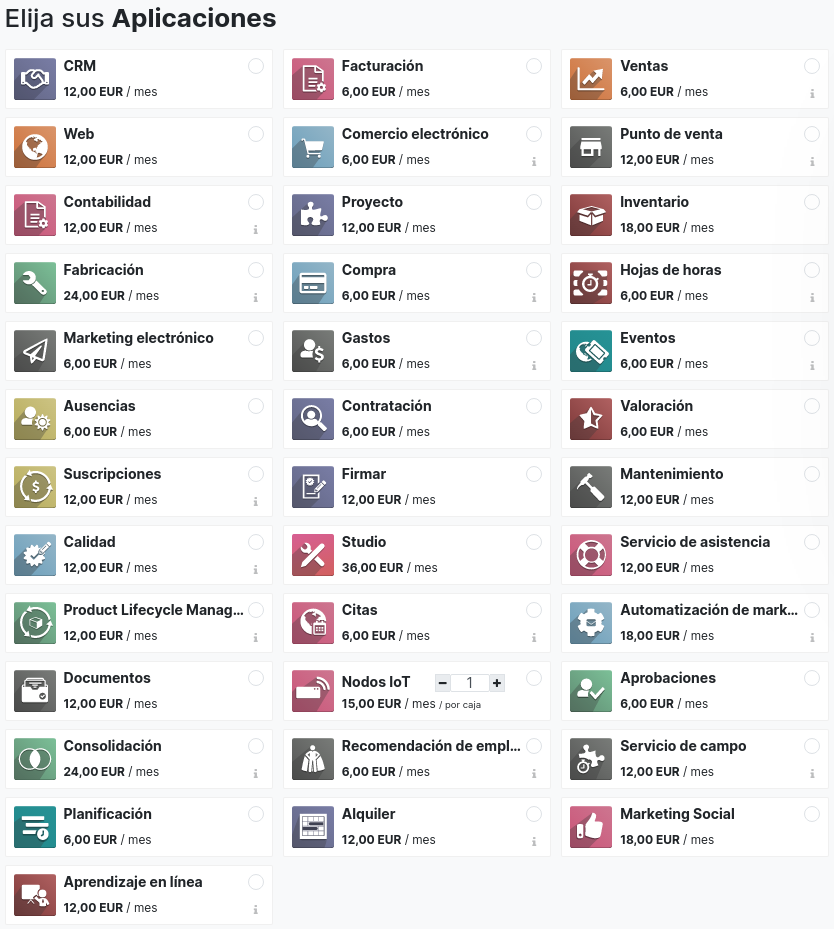
\includegraphics[scale=0.4]{archivos/odooModules.png}
\end{tabular}
\caption{Compra de módulos de Odoo}
\label{fig:odooModules}
\end{figure}
\clearpage
\begin{figure}[h]
\centering
\begin{tabular}{ccc}
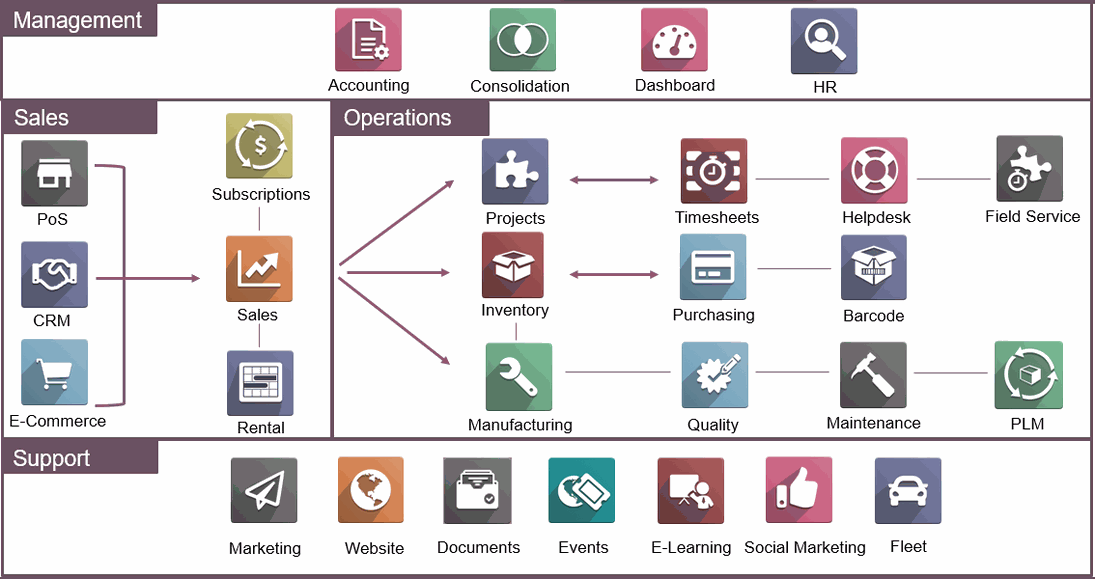
\includegraphics[scale=0.38]{archivos/odooModules2.png}
\end{tabular}
\caption{Comunicación entre módulos de Odoo}
\label{fig:odooModules}
\end{figure}
\par Podríamos listar las siguientes ventajas:
\begin{itemize}
    \item Bajo coste
    \item Open source
    \item Capacidad de operar en la nube
    \item Inyección de módulo hechos a mano
\end{itemize}
Y las siguientes desventajas:
\begin{itemize}
    \item Tiene coste
    \item Necesita mantenimiento informático avanzado
    \item Curva de aprendizaje y estudio de módulos para la adopción
\end{itemize}
\vspace{0.5em}
\par A pesar de tener ventajas en la instalación y puesta en marcha frente a otras soluciones como \citep{oracleERP} o \citep{sapERP}, y a pesar de ser open source con una comunidad amplia de desarrolladores y con miles de aplicaciones; sigue siendo demasiado complejo para lo que necesitamos, la propia plataforma recomienda contactar con un distribuidor para que ayude al negocio a implantar la solución dado que hacen falta conocimientos informáticos extensos. Recordamos que pretendemos una solución simple de usar y poner en marcha.
\vspace{0.5em}
\par Por lo que terminamos por descartar las soluciones ERP que el mercado pone a nuestra disposición. Las necesidades del economato social son muy concretas y decidimos que hacer ad hoc una solución verdaderamente libre nos resuelve el problema que tenemos, además de permitirnos escalar y mantener la aplicación de forma libre si la solución saltase a otros bancos de alimentos.
% --------------------------------------------------------------
% --------------------------------------------------------------
% --------------------------------------------------------------
\clearpage
\subsection{Decidiendo arquitectura}
Dadas las premisas de arquitectura, para este proyecto optamos por estudiar las siguientes posibilidades:
\begin{itemize}
    \item Raspberry pi y Do It Yourself
    \item Computación elástica bajo demanda
    \item Serverless
\end{itemize}
% --------------------------------------------------------------
% --------------------------------------------------------------
% --------------------------------------------------------------
\subsubsection{Raspberry pi (DIY)}
\begin{figure}[h]
\centering
\begin{tabular}{ccc}
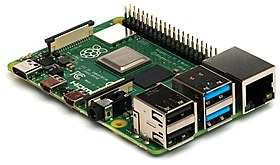
\includegraphics[scale=0.5]{archivos/RPi_4.jpg}
\end{tabular}
\caption{Raspberry Pi 4 Modelo B}
\label{fig:rpi4}
\end{figure}
\vspace{1em}
\par La Raspberry Pi fue nuestra primera idea, debido a su condición de software de código abierto, bajo coste de adquisición, reducido espacio y poco consumo.
\vspace{1em}
\par La Raspberry Pi es una serie de ordenadores de placa reducida de bajo coste desarrollado en el Reino Unido. Su objetivo principal ha sido siempre poner a disposición de todo el mundo el poder de la informática con un ordenador reducido en espacio y coste. Cuando se creó, se pretendía promocionar la enseñanza informática en las escuelas, pero terminó siendo mucho más popular de lo que se esperaba. Como se muestra en la figura 2.3, no trae ningún tipo de periférico, ni carcasa; aunque ya hay packs de todo tipo para ayudar a la adopción del hardware.
\begin{figure}[h]
\centering
\begin{tabular}{ccc}
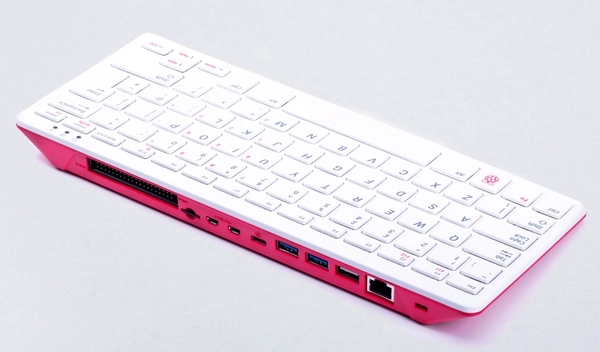
\includegraphics[scale=0.4]{archivos/rpi4keyboard.png}
\end{tabular}
\caption{Raspberry Pi integrada en el interior de un teclado}
\label{fig:rpi4keyboard}
\end{figure}
\begin{figure}[h]
\centering
\begin{tabular}{ccc}
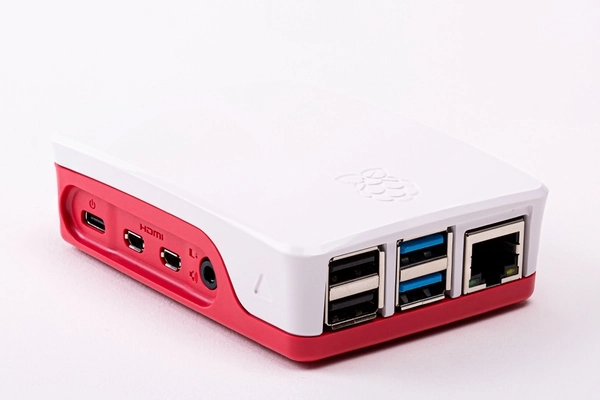
\includegraphics[scale=0.4]{archivos/rpi4case.png}
\end{tabular}
\caption{Raspberry Pi protegida con funda}
\label{fig:rpi4case}
\end{figure}
\vspace{1em}
\par En cuanto a la distribución del hardware, la Raspberry Pi Foundation no indica expresamente que el hardware sea libre o con derechos de marca, aunque sí explican en su web oficial que cualquiera puede convertirse en revendedor o redistribuidor de las tarjetas Raspberry Pi, dando a entender que es un producto con propiedad registrada pero permitiendo el uso libre tanto a nivel educativo como particular.
\vspace{1em}
\par Su software sí es código abierto, basando su sistema operativo en Debian y llamándose Raspberry Pi OS; el procesador es ARM por lo que la paquetería debianita tiene que pasar un proceso de adaptación y recompilación para poder usarse en la Pi OS.
\vspace{1em}
\par Todas estas características fueron las que nos incitó a considerarla como una buena solución a lo que se no estaba planteando. Pero el conocimiento de sistemas informáticos iba a ser una carga muy elevada en caso de avería, mantenimiento o escalabilidad. Además, una última idea nos hizo deshacernos de las Pis como solución de hardware, la disponibilidad del software.
\vspace{1em}
\par Una de nuestras premisas era tener en cuenta la capacidad de salto a otros bancos de alimentos, tanto de la zona, como de la ciudad; haber resuelto el host de la aplicación web en una raspberry pi nos habría planteado problemas de arquitectura mucho más elevados más adelante.
\begin{itemize}
    \item ¿Dónde deberá localizarse el servidor una vez haya más de una sede haciendo uso?
    \item ¿Deberíamos distribuir su ejecución por si el nodo principal se queda sin luz?
\end{itemize}
En seguida caímos en que si bien es una problemática resoluble, teníamos soluciones al alcance de la mano y por muy bajo coste: Los servicios de computación en la nube bajo demanda.
% --------------------------------------------------------------
% --------------------------------------------------------------
% --------------------------------------------------------------
\clearpage
\subsubsection{Computación elástica bajo demanda (Cloud)}
Dado que la arquitectura hardware mantenida por nosotros no iba a ser viable a la larga, pusimos la vista en la computación elástica.
\vspace{1em}
\par Los servicios Cloud nacen para dar una recurso muy simple de explicar y no tan fácil de proveer, capacidad de procesamiento infinita. Un servicio cloud no es simplemente un software que corre en el ordenador de otro en lugar del propio, es la escalabilidad (casi) sin límites y bajo demanda, lo que le da potencia como idea. Hoy en día hay múltiples proveedores de servicios cloud, aunque los jugadores más fuertes son indiscutiblemente Aws, Azure y Digital Ocean.
\begin{table}[h]
\centering
\begin{tabular}{ccc}

\includegraphics[scale=0.2]{archivos/aws.png}

\includegraphics[scale=0.2]{archivos/azure.png}

\includegraphics[scale=0.08]{archivos/digitalocean.png}
\end{tabular}
\end{table}
\vspace{1em}
\par Dado que yo tengo experiencia laboral y personal como arquitecto cloud en servicios aws y me estoy preparando el examen oficial, decidimos sin pensárnoslo mucho en estudiar nuestra solución como nativa cloud haciendo uso de los servicios Aws. Si bien Aws tiene capas gratuitas, éstas son temporales en caso de la computación y son circulares en caso de la transmisión de datos. Dado nuestro cliente y nuestro estudio de casos de uso, sabíamos que podríamos usar las capas gratuitas de transferencia de datos sin problema, pero el hosting sí podría suponer una traba. Aún así, proseguimos.
\vspace{1em}
\par En concreto, con Aws, usaríamos una de las máquinas de computación elástica más pequeña que tiene, para montar nuestro servidor web, haciendo uso de imágenes dockerizadas y distribuídas por el propio registro de imágenes de Aws. En todo momento hemos querido mantener el estándar y el open source, esto facilitaría la recepción de voluntarios informáticos. Las máquinas que Aws provee, servicio llamado \citep{ec2AWS}, es descrito como `Capacidad informática segura y de tamaño ajustable que admite prácticamente cualquier carga de trabajo`.
\vspace{1em}
\par La parte buena de usar este servicio es la capacidad de usar sus servicios bajo demanda, podemos hacer crecer y disminuir máquinas conforme necesitemos, balancear la carga entre varios nodos si quisiéramos o incluso aumentar nuestro porcentaje de disponibilidad usando la Route 53 para que si una región deja de estar disponible, automáticamente el trafico quedase redirigido a la región más cercana. Habríamos usado una base de datos adhoc RDS para evitar configuración y mantenimiento, teniéndolo todo centralizado en una misma red para minimizar la espera por latencia y habríamos protegido el acceso y ddos de nuestra máquina usando el servicio de ApiGateway. El frontend podría ser desatendido, almacenado en un S3 de bajo coste y distribuido y cacheado por el servicio de CloudFront.
\begin{figure}[h]
\centering
\begin{tabular}{ccc}
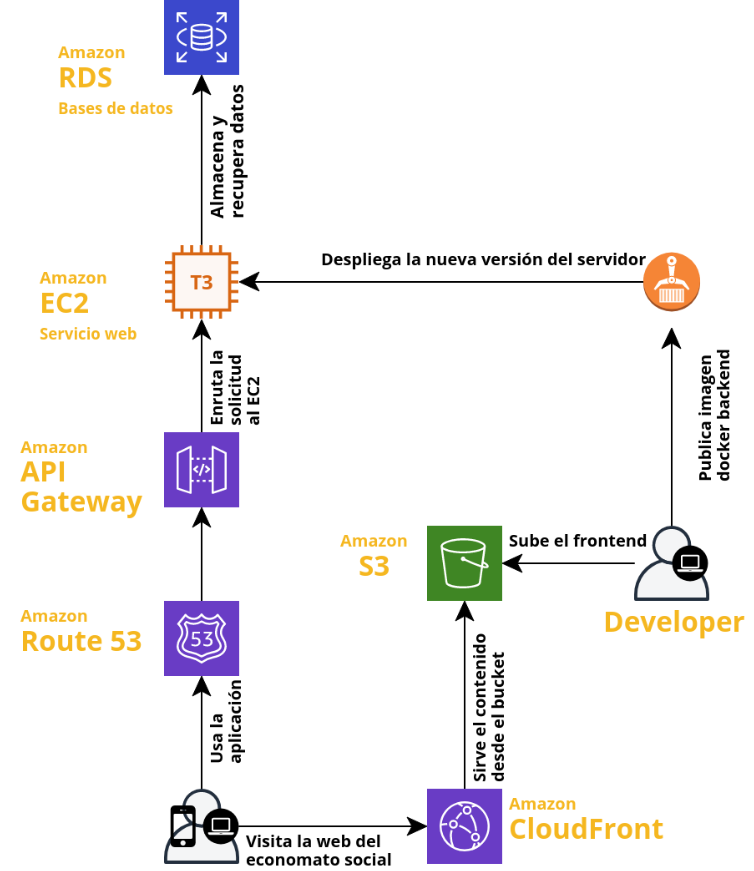
\includegraphics[scale=0.5]{archivos/arquitecturaAws.png}
\end{tabular}
\caption{Arquitectura simplificada}
\end{figure}
\clearpage
\begin{figure}[h]
\centering
\begin{tabular}{ccc}
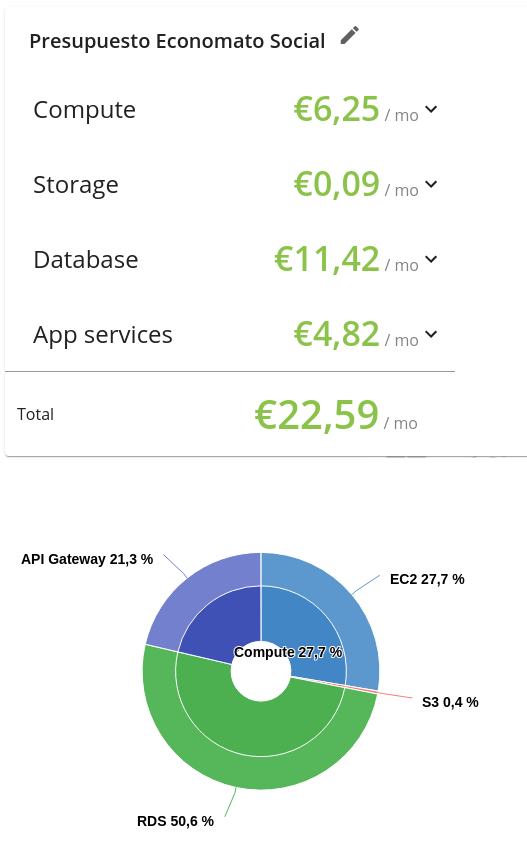
\includegraphics[scale=0.6]{archivos/budgetAws.png}
\end{tabular}
\caption{Presupuesto simplificado}
\end{figure}
\clearpage
\vspace{1em}
\par Todo esto hace de la arquitectura un proyecto ideal, una estructura sencilla de manejar para alguien con conocimientos, pero aunque hubiésemos podido aceptar el presupuesto, volvimos a toparnos la misma problemática que con la Raspberry Pi. ¿Qué ocurriría si una máquina deja de estar accesible? ¿Y si hay un problema en la configuración de red o de acceso por grupos de seguridad? ¿Y si alguien toca sin querer algo que no debe en un despliegue? Nuestro objetivo de no ceder el mantenimiento a la posibilidad de tener siempre conocimientos informáticos disponibles en el voluntariado, era más fuerte que intentar idear una arquitectura digna de proyectos modernos.
\vspace{1em}
\par Sólo nos quedaba una carta que jugar, una forma de explotar el cloud que ya había usado en proyectos anteriores, y que podría ser lo que nos permitiese centrar el conocimiento informático voluntario en el desarrollo y mantenimiento de la aplicación; permitiéndonos ignorar la disponibilidad del servicio y configuración de las máquinas: el Serverless.
% --------------------------------------------------------------
% --------------------------------------------------------------
% --------------------------------------------------------------
\clearpage
\subsubsection{Serverless (Cloud)}
Como ya hemos ido hablando, el sector privado tiende cada vez hacia la nube, sobretodo el sector comercial; dada la capacidad de contratar y configurar soluciones a medida de las necesidades de cada uno. Dentro de la oferta de servicios cloud existe el uno llamado Serverless Computing, una de las prácticas más recientes, y comúnmente conocido como FaaS (Function as a Service).
\vspace{1em}
\par El primer concepto que nos atrajo para adoptar esta solución es la propia descripción del Serverless Computing o Arquitectura Serverless. Éste viene a ser un modelo que permite a los usuarios crear y ejecutar aplicaciones y procesos sin entrar en contacto con el servidor subyacente. Dado que es justo lo que queremos, un entorno en la nube en el que es el propio proveedor el que se ocupa del suministro, gestión y escalado del servicio. Ésto además tiene un punto fuerte para nuestra intención de adopción futura, podemos centrar toda nuestra atención y esfuerzo en el desarrollo y en la ejecución del software, ahorrando tareas y conocimientos al equipo implicado.
\vspace{1em}
\par También, normalmente los proveedores de Serverless no sólo son responsables de que los recursos de servidor estén siempre disponibles, si no también lo son de garantizar la disponibilidad del servicio; es decir, seguridad anticaída. Normalmente este tipo de servicios tienen un modelo de pago por uso, el cual abordaremos después.
\subsubsection{¿Cómo funciona?}
En una infraestructura serverless, la gestión del hardware por parte del proveedor es esencial. El único desafío con el que tienen que lidiar los usuarios es integrar su software o su lógica, incluidas las funciones adecuadas, en el espacio alquilado en la nube. El acceso a estas funciones se puede realizar de dos maneras:
\begin{itemize}
    \item de forma asíncrona, a través de eventos
    \item de forma síncrona, según el modelo Cliente-Servidor clásico
\end{itemize}
\vspace{1em}
\par La forma de uso asíncrona ofrece la ventaja de evitar acoplamiento entre las funciones y mantener la demanda de recursos en un nivel bajo durante la ejecución. Un ejemplo de función asíncrona sería que al cargar una imagen cree también un icono en miniatura. Son funciones atómicas, que permiten mucho control en el código, simplicidad y reducción de gastos, dado que sólo se paga cuando se usa; problemas de optimización también son más fáciles de acotar y se puede decidir poner recursos a optimizar una función que funcione deficientemente pero no necesariamente a todo el sistema.
\vspace{1em}
\par El uso que nosotros vamos a darle al Serverless es la función síncrona, vamos a usar el servicio para poder mantener levantado un servidor web sin tener que estar pendientes de mantener el sistema, actualizarlo o configurarlo. En concreto, vamos a usar la solución que provee Heroku, un proveedor de servicios Serverless con una generosa capa gratuita que a éste trabajo le vendrá de perlas. La única limitación que pueda importarnos, de las que tiene Heroku en su capa gratuita, es que los servicios mueren tras 5 minutos sin uso; haciendo que la siguiente petición tarde un poco más. Esto encaja a la perfección con nuestras necesidades pues, a priori, se le va a dar uso al sistema un par de días a la semana.
\vspace{1em}
\par A diferencia de una infrastructura de plataforma como servicio, el proveedor Serverless no facilita para ello un entorno de trabajo duradero para todo el tiempo de trabajo, si no que aporta de manera puntual y en tiempo real aquellos recursos que se requieren durante el tiempo de ejecución de la llamada a la función. A pesar de llamarse Serverless, obviamente sí hay servidores detrás del telón, aunque el usuario nunca lo perciba.
\subsubsection{Vista general de ventajas y desventajas}
Las infraestructuras convencionales en la nube permiten al usuario administrar y eliminar el hardware que se require pero, a menudo, ésto requiere grandes esfuerzos a nivel de administración y microgestión. Lo que pretende el Serverless es minimaz eso al máximo.
\vspace{1em}
\par Podríamos considerar las siguientes ventajas y desventajas
\begin{itemize}
    \item Ventajas
    \begin{itemize}
        \item Escalamiento y administración de los recursos necesarios por parte del proveedor
        \item Suministro ágil de los recursos en tiempo real, en función del consumo en cada momento
        \item Cobro únicamente por uso al milisegundo
        \item Gran tolerancia a errores gracias a la infraestructura flexible de hardaware
    \end{itemize}
    \item Desventajas
    \begin{itemize}
        \item Acceso restringido a los sistemas e incapacidad de configuración de éstos
        \item Grandes proyectos basados en funciones asíncronas pueden suponer un gran esfuerzo de implementación
        \item Gran dependencia del proveedor, posibles dificultades de migración
        \item Procesos de monitorización y depuración de errores más complejos
    \end{itemize}
\end{itemize}
\subsubsection{Cuándo se usa el principio Serverless}
El serverless computing ha sido concebido principalmente para el intercambio efímero de datos de aplicaciones web y de negocios en la nube, aunque acabó abarcando servicios más complejos y con una vida de ejecución más larga pero basándose en las mismas premisas: escalabilidad elástica en tiempo real y adecuándose al uso, sin que el usuario tenga que hacerse cargo de configuraciones de sistemas y redes.
\vspace{1em}
\par Los escenarios más comunes del Serverless son los siguientes:
\begin{itemize}
    \item Proxy API: muchas aplicaciones comerciales antiguas cuenta con interfaces complejas y lentas. Mediante el serverless se puede crear una capa de abstracción alternativa para poder acceder a estas aplicaciones mediante una API REST mucho más simple
    \item Serverless Backend: el serverless computing también se usa cada vez más para construir y soportar todo el backend de una aplicación en la nube. Backend as a Service.
    \item Procesamiento de datos no estructurados: hoy en día, es imposible imaginar un entorno de negocios sin big data. En este contexto, el serverless se muestra como un gran aliado para procesar este tipo de información.
    \item Ejecución de tareas según horario: una gran cantidad de demanda de este tipo de funciones en un horario definido, un disparador que ejecuta alguna automatización aislada como backups de bases de datos, reorganización de datos, etc.
    \item Aplicación de asistentes y chat bots: Normalmente este tipo de aplicaciones son sin estado y conectan con servicios de modelos inteligentes más complejos, estas interfaces en serverless están en auge.
\end{itemize}
% --------------------------------------------------------------
% --------------------------------------------------------------
% --------------------------------------------------------------
\subsubsection{Ejemplos de uso con heroku}
\begin{figure}[h]
\centering
\begin{tabular}{ccc}
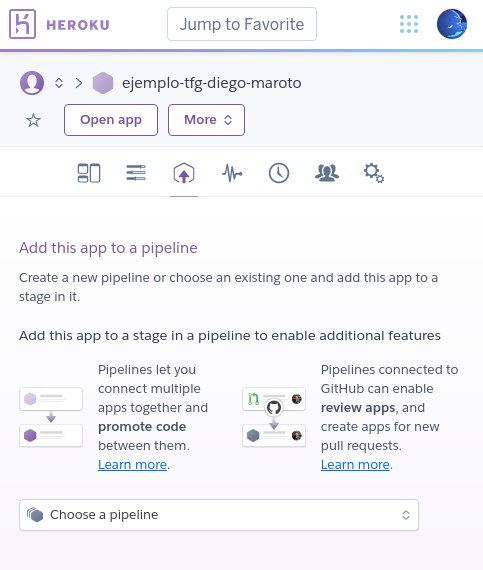
\includegraphics[scale=0.5]{archivos/heroku01.png}
\end{tabular}
\caption{Configurando proyecto en Heroku}
\end{figure}

\begin{figure}[h]
\centering
\begin{tabular}{ccc}

\includegraphics[scale=0.5]{archivos/heroku02.png}
\end{tabular}
\caption{CI/CD en Heroku}
\end{figure}

\begin{figure}[h]
\centering
\begin{tabular}{ccc}
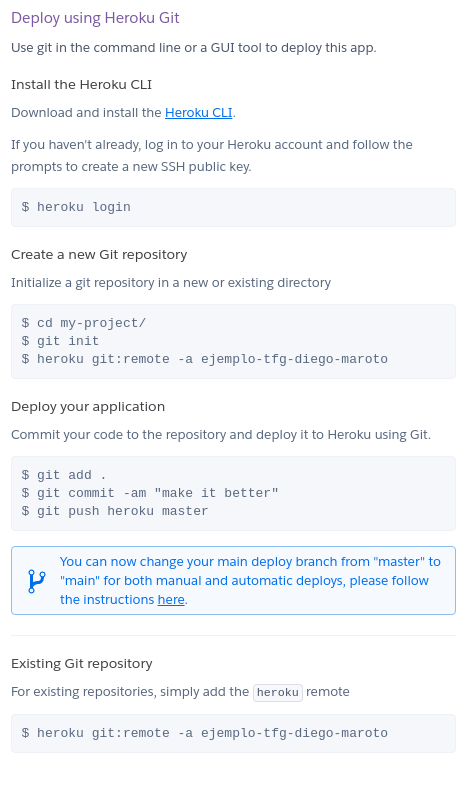
\includegraphics[scale=0.5]{archivos/heroku03.png}
\end{tabular}
\caption{Ejemplo de uso de Heroku por línea de comandos}
\end{figure}
\clearpage
% --------------------------------------------------------------
% --------------------------------------------------------------
% --------------------------------------------------------------
\clearpage
\subsection{Stack FrontEnd/BackEend}
Una de nuestras principales preocupaciones, como se lleva diciendo toda la exposición, es la escalabilidad del proyecto en cuanto a la facilidad de colaboración técnica voluntaria. Desde esta premisa estuvimos estudiando qué lenguajes de programación podrían encajar en esta dinámica.
\vspace{1em}
\par Del mundo del desarrollo, la plataforma más usada de largo es Stack Overflow; en esencia es un foro tecnológico donde usuarios escriben sus dudas y otros usuarios intentan resolverlas. Stack Overflow hace una encuesta todos los años para extraer datos demográficos, económicos y tecnológicos sobre la comunidad tecnológica mundial. Decidimos basarnos en la encuesta de 2020 \citep{techSurveyStackOverflow} para valorar el stack a usar.
\vspace{1em}
\par Como se aprecia en la encuesta, javascript es el más usado tanto profesional como amateur; además, encaja en nuestra idea inicial, en la que considerábamos usar el mismo lenguaje para frontend y backend una ventaja competitiva. Dado que va a ser un proyecto dilatado en el tiempo, un lenguaje de tipado estático sería una buena forma de agilizar la curva de aprendizaje del proyecto y recortar la barrera de entrada para los aspirantes; así pues, dado que Typescript está en el top 10 y podemos considerarlo javascript, optamos por usarlo.
\vspace{1em}
\par Una vez decidido el lenguaje, queda la decisión de si usar frameworks o no. No usar frameworks puede ser potente en un inicio pues permite la flexibilidad de montar el sistema como se quiera y definir unas pautas; unas pautas que preferiríamos que pudiesen ponerse en tela de juicio lo menos posible, así que optaremos por frameworks pues así la forma de hacer las cosas será siempre la misma independientemente de quién trabaje en el proyecto.
\vspace{1em}
\par En javascript es muy común el stack MEAN (Mongo, Express, Angular y Nodejs), y para acomodar el backend y el frontend, usaremos para el backend con Express el framework Nestjs; un framework disponible en typescript cuya estructura MVC es muy parecida a Angular, de esta forma, un desarrollador frontend podrá pivotar al backend y viceversa con muy poco problema.
\vspace{1em}
\par Para la persistencia de datos se había propuesto MongoDB desde un inicio, y éste encaja con Javascript a la perfección, dado que los documentos de ambos se anotan en JSON, la integración entre ambos es intuitiva y sencilla. Además, MongoDB tiene capa gratuita en su servicio cloud Compass y es justo lo que queremos. 
\vspace{1em}
\par Y de esta forma queda decidido, se usará Typescript con Nestjs para el backend, Typescript con Angular para el frontend y MongoDB para la persistencia de datos. 
\clearpage
% --------------------------------------------------------------
% --------------------------------------------------------------
% --------------------------------------------------------------